\chapter{Desenho do Processo Macro} \label{cha:desenhomacro}
Neste capítulo são apresentados os diagramas de atividades das principais funcionalidades que serão implementados no aplicativo.

%DUVIDA: MTO PEQUENO SÓ ATIVIDADES?

A atividade "Buscar Produto", diagramada na figura \autoref{fig:atividade_comparar}, na qual o usuário insere um termo de pesquisa para encontrar produtos de interesse. Em seguida, o sistema executa a ação de "Pesquisar Produto", onde são consultadas as localizações cadastradas para encontrar produtos que correspondam ao termo de pesquisa. Após a pesquisa, o sistema verifica se foram encontrados produtos. Se sim, o fluxo segue para a atividade "Comparar Preços", na qual os preços dos produtos encontrados são coletados e comparados entre as diferentes localizações ou fontes disponíveis. Durante essa comparação, o sistema identifica o melhor preço para cada produto.

Ao final da atividade de comparar preços, o sistema pode exibir os resultados da comparação ao usuário, mostrando os produtos encontrados, seus preços em diferentes localizações e destacando o melhor preço disponível. Isso ajuda o usuário a tomar uma decisão informada sobre qual produto comprar com base no preço mais atrativo.

A atividade de cadastrar produtos, diagramada na figura \autoref{fig:cadastrar_produtos}, tem início na etapa de buscar de produtos. O usuário seleciona a opção de cadastro e tem duas possibilidades, inserir o produto manualmente ou escanear uma nota fiscal. A inserção manual se da por um simples formulário de cadastro enquanto pela nota fiscal o sistema identifica todos os produtos relacionados a mesma e os cadastra no sistema após uma confirmação do usuário.

\imagem{DIAGRAMA DE ATIVIDADES COMPARAR PREÇOS}{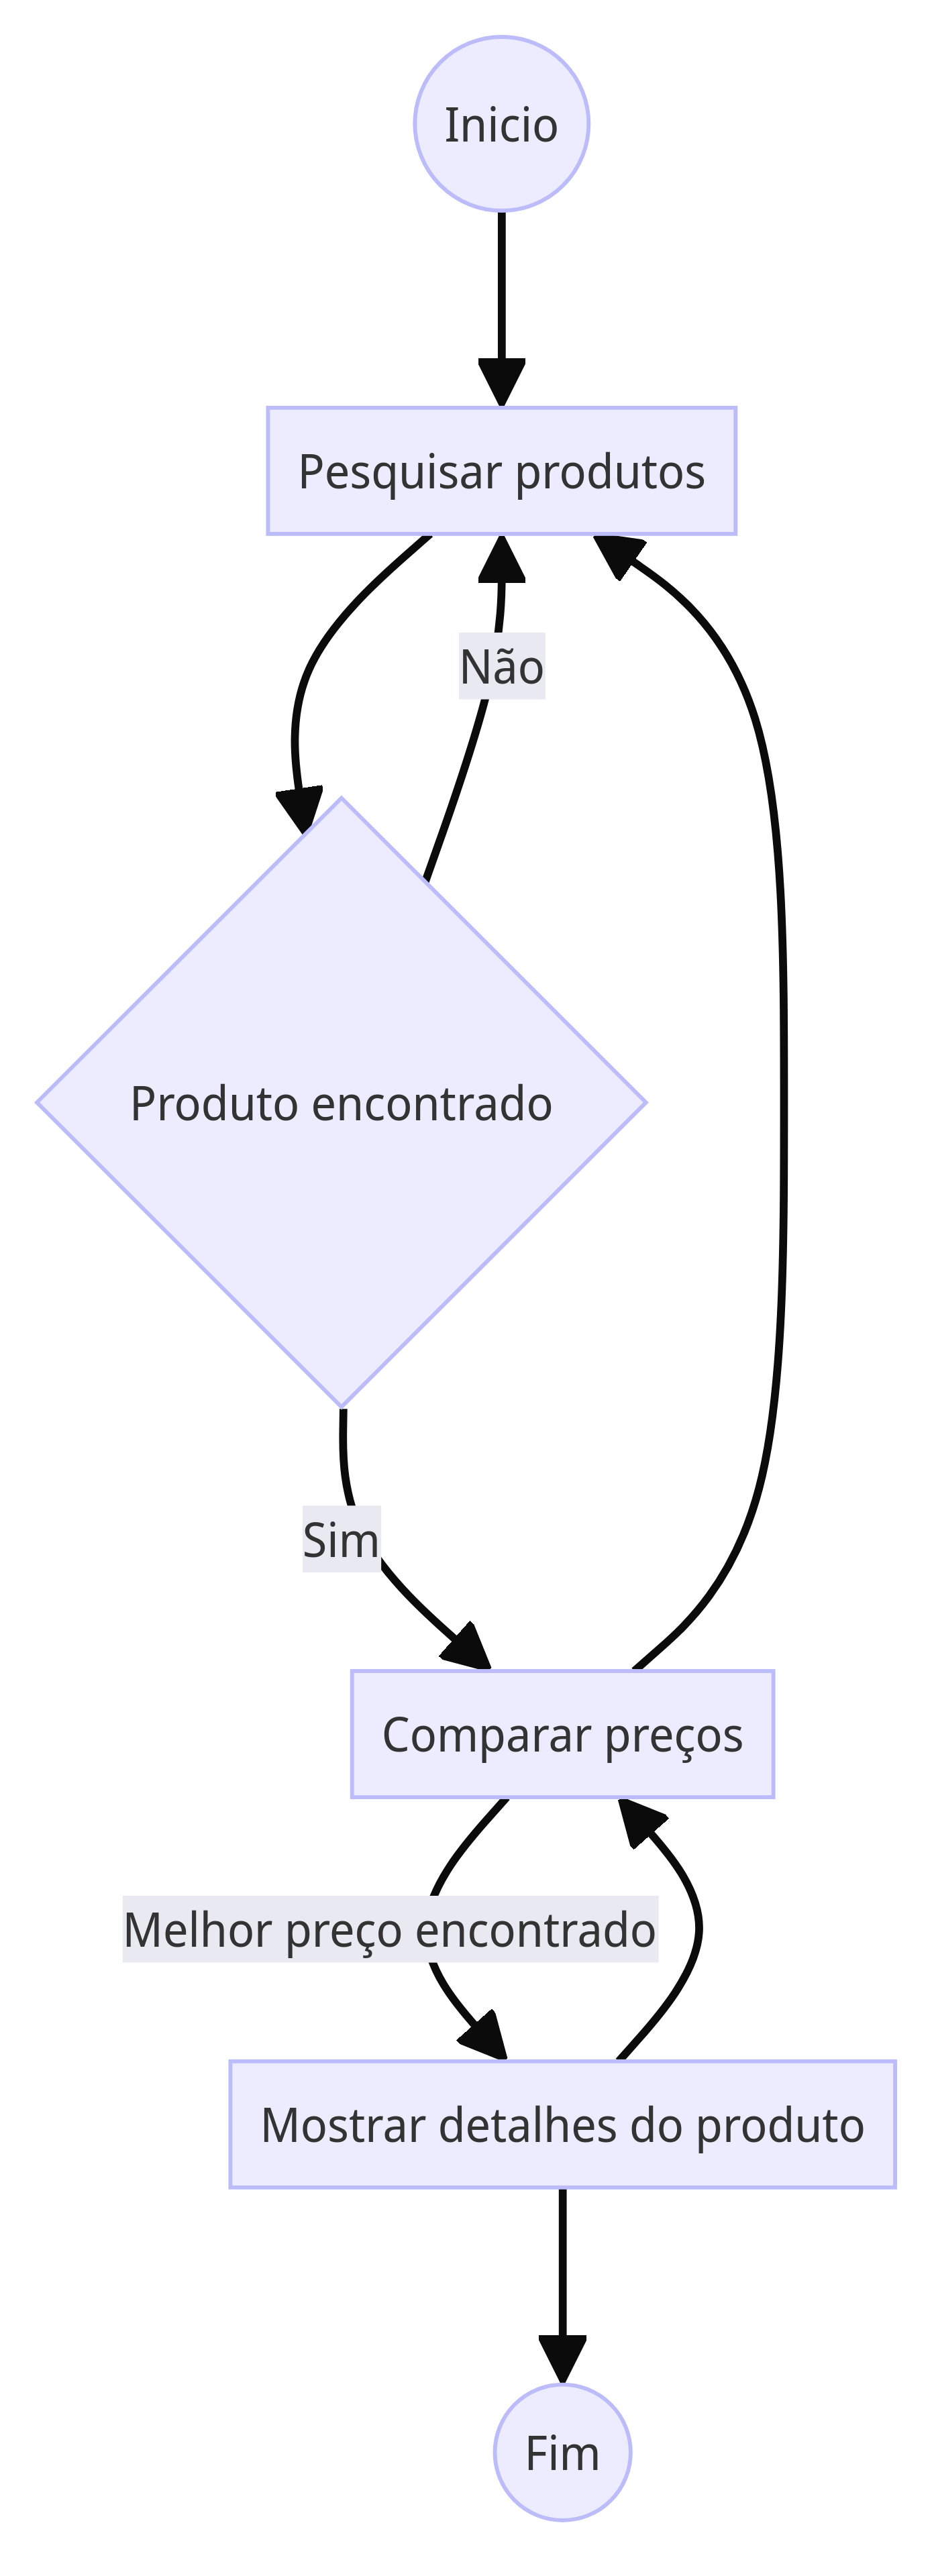
\includegraphics[width = 150mm]{fig/atividade/atividade1.png}}{O Autor (2024)}{atividade_comparar}{nota(s)}{legenda(s)}

\imagem{DIAGRAMA DE ATIVIDADES CADASTRAR PRODUTOS}{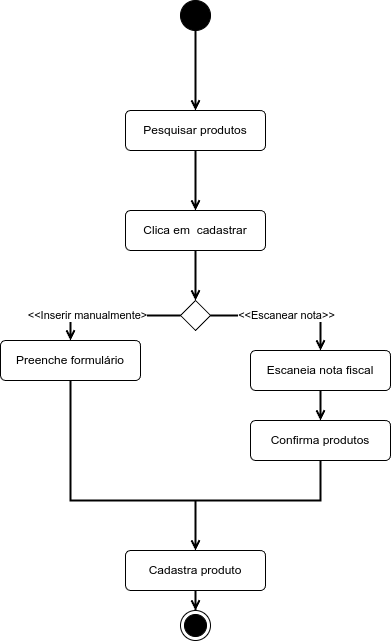
\includegraphics[width = 120mm]{fig/atividade/atividade2.png}}{O Autor (2024)}{cadastrar_produtos}{nota(s)}{legenda(s)}